\documentclass{beamer}

\usepackage{beamerthemesplit}
\usepackage{verbatim}

\usepackage{xcolor}
\definecolor{mygray}{RGB}{200,200,200}
\usetheme{default}
%\usetheme{Pittsburgh}
%\usecolortheme{seagull}
%\usecolortheme{seahorse}
%\usecolortheme{beaver}
\usecolortheme{mule}

\usefonttheme{serif}

%\DeclareGraphicsExtensions{.pdf,.png,.jpg}

\newcommand{\snT}{$(S/N)_{\textrm{size}}$}
%\newcommand{\snT}{$\left( \frac{S}{N}\right)_{\textrm{size}}$}
\newcommand{\snflux}{$(S/N)_{\textrm{flux}}$}
%\newcommand{\snflux}{$\left( \frac{S}{N}\right)_{\textrm{flux}}$}

\newcommand{\lensfit}{\texttt{LENSFIT}}
\newcommand{\numba}{\texttt{Numba}}
\newcommand{\python}{\texttt{Python}}
\newcommand{\ngmix}{\texttt{ngmix}}
\newcommand{\shear}{{\bf g}}
\newcommand{\redmapper}{redMaPPer}

\newcommand{\prelim}{{\bf{\it Preliminary}}}

\definecolor{gold}{rgb}{1.,0.84,0.}


\title{The Dark Energy Survey}
\author{Erin Sheldon}
\institute{Brookhaven National Laboratory}

% http://texblog.net/latex-archive/plaintex/beamer-footline-frame-number/
% to add the page (frame ) number and not screw up the bottom line
% works for split themes?
\expandafter\def\expandafter\insertshorttitle\expandafter{%
      \insertshorttitle\hfill%
        \insertframenumber\,/\,\inserttotalframenumber}

% suppress navigation bar
\beamertemplatenavigationsymbolsempty
\setbeamertemplate{footline}{}

\begin{document}

\frame{\titlepage}

\usebackgroundtemplate{%
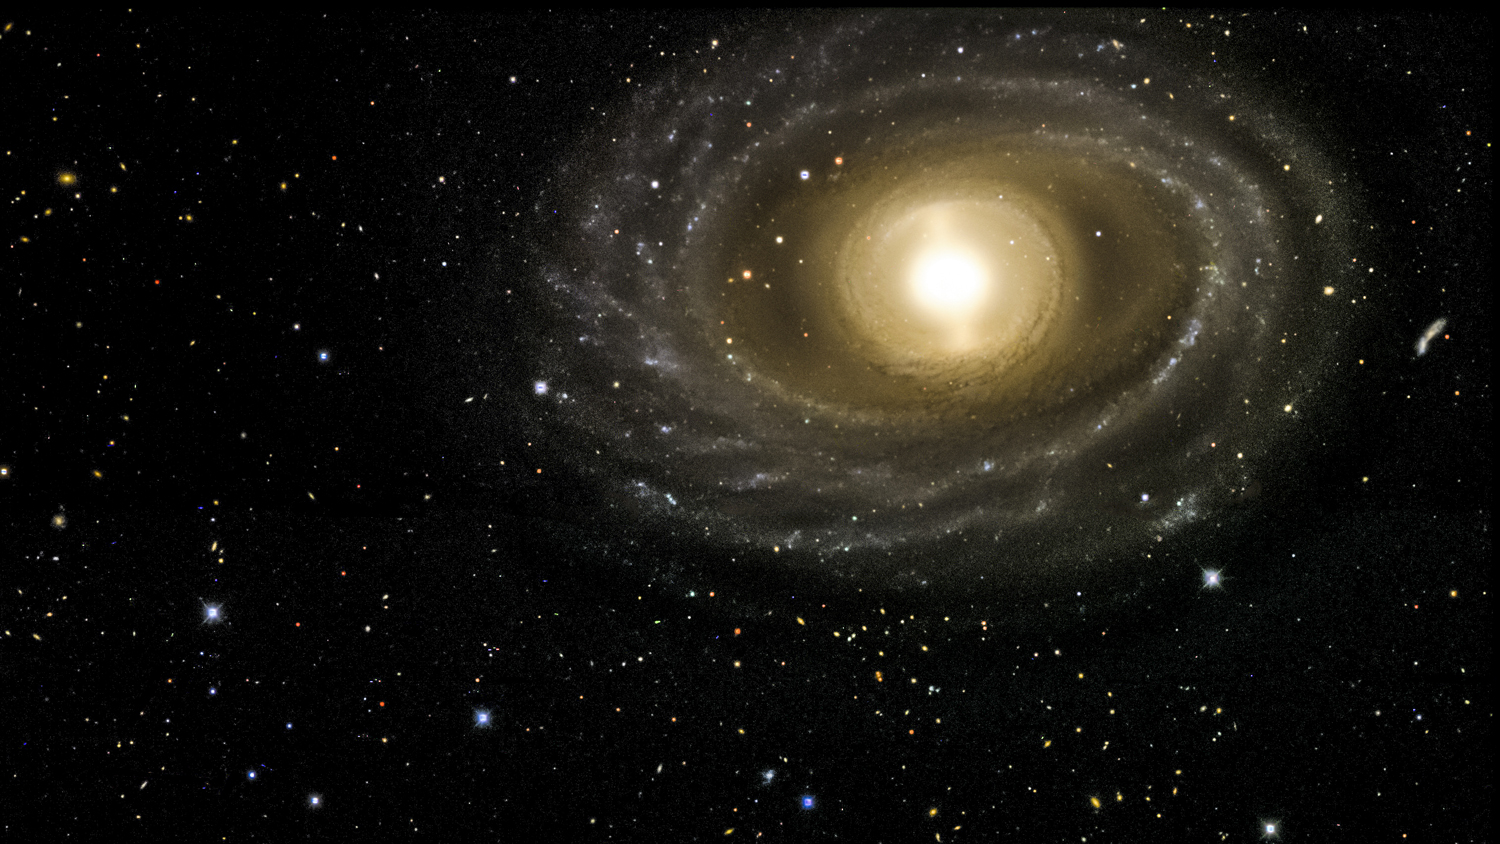
\includegraphics[trim=100 0 0 0,clip,height=\paperheight]{DES-2013-01-medres.jpg}}
\frame
{
}


\setbeamertemplate{background canvas}[vertical shading][bottom=mgray,top=mblack]

\frame
{
    \frametitle{Outline}

    \setbeamerfont*{itemize/enumerate body}{size=\Large}
    \setbeamerfont*{itemize/enumerate subbody}{parent=itemize/enumerate body}
    \setbeamerfont*{itemize/enumerate subsubbody}{parent=itemize/enumerate body}
 
    \begin{itemize}

        \item The Primary Goal is to Study Dark Energy
        \item First I'll Give Some Background
        
        \begin{itemize}
            \item Cosmology
            \item Dark Energy
            \item Gravitational Lensing: a tool to study dark energy
        \end{itemize}

        \item Dark Energy Survey

        \begin{itemize}
            \item{Survey Design}
            \item{First Results From 2015}
        \end{itemize}

        \item Current Research

    \end{itemize}

}

\frame
{
    \frametitle{Cosmology}

    \setbeamerfont*{itemize/enumerate body}{size=\Large}
    \setbeamerfont*{itemize/enumerate subbody}{parent=itemize/enumerate body}
    \setbeamerfont*{itemize/enumerate subsubbody}{parent=itemize/enumerate body}
 
    \begin{itemize}

        \item The study of the contents and evolution of the universe
        
        \begin{itemize}
            \item Observe the universe in as many
                ways as we can
            \item Explain what we know in terms of fundamental physics
        \end{itemize}

    \end{itemize}

}

{
    \definecolor{mblack}{RGB}{0,0,0}
    \setbeamertemplate{background canvas}[vertical shading][bottom=black,top=black]

    \frame
    {	

        \begin{center}
            %\includegraphics[trim=left bottom right top, clip]{file}
            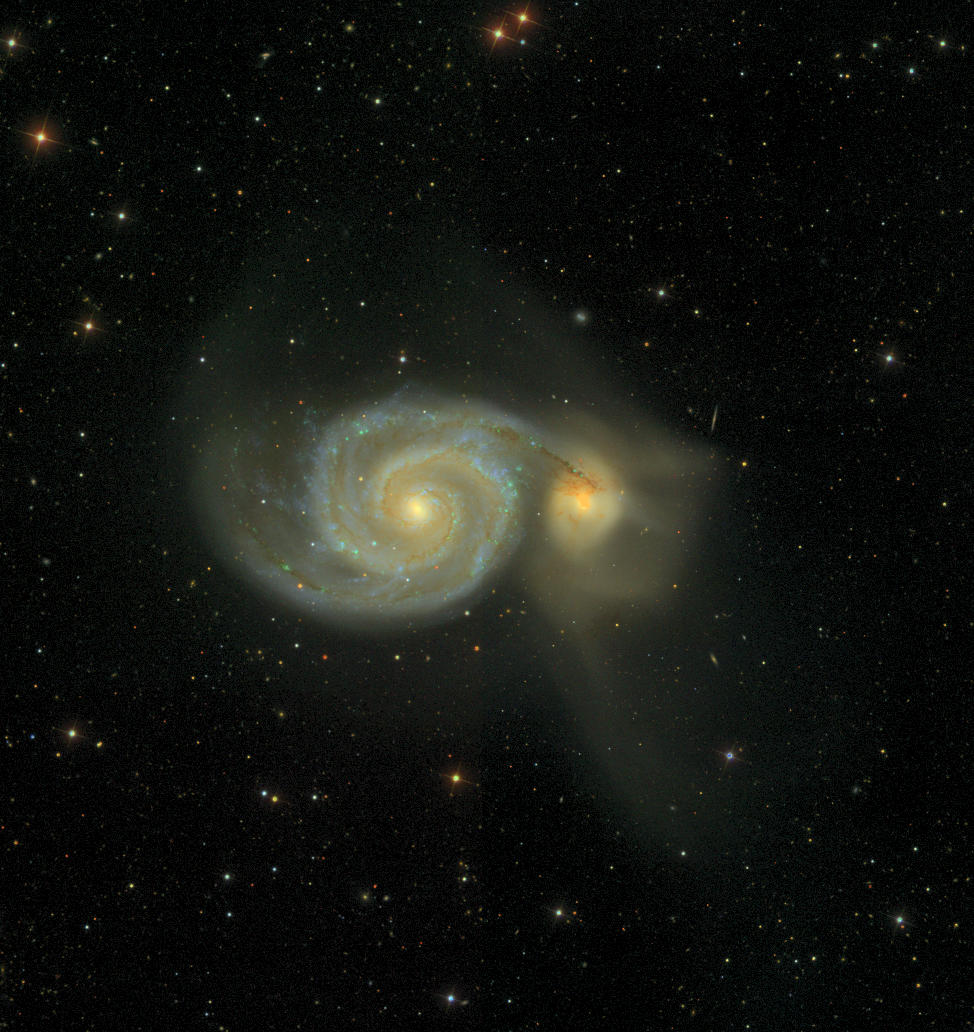
\includegraphics[trim=0 0 0 100,clip,width=0.85\textwidth]{M51-4x4.jpg}
            \newline
            \hfill {\tiny M51 ``Whirlpool Galaxy'', SDSS/Robert Lupton}
        \end{center}

    }
    \definecolor{mblack}{RGB}{50,50,50}
    \setbeamertemplate{background canvas}[vertical shading][bottom=mgray,top=mblack]
}

{
    \definecolor{mblack}{RGB}{0,0,0}
    \setbeamertemplate{background canvas}[vertical shading][bottom=black,top=black]

    \frame
    {	

        \begin{center}

        \centerline{\includegraphics[trim=0 400 0 500,clip,width=\paperwidth]{M104b_peris2048.jpg}}
            \hfill {\tiny M104, ``Sombrero'', NASA/ESA/V. Peris}
        \end{center}
    }
    \definecolor{mblack}{RGB}{50,50,50}
    \setbeamertemplate{background canvas}[vertical shading][bottom=mgray,top=mblack]
}




{
    \definecolor{mblack}{RGB}{0,0,0}
    \setbeamertemplate{background canvas}[vertical shading][bottom=black,top=black]


    \frame
    {
        \begin{center}
             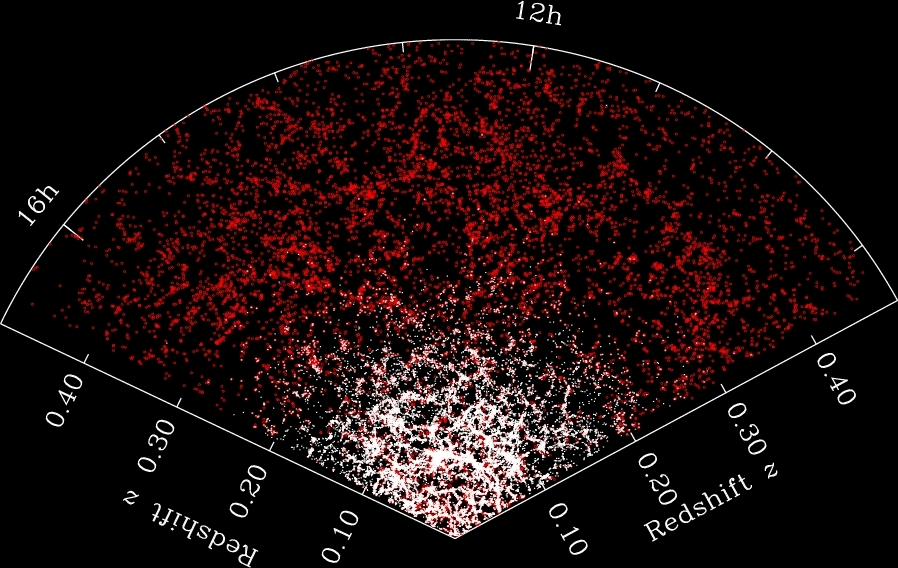
\includegraphics[width=\textwidth]{sdss-gals-blanton.jpg}
         \end{center}
        {\tiny \hfill SDSS Galaxies (M. Blanton)}
    }
    \definecolor{mblack}{RGB}{50,50,50}
    \setbeamertemplate{background canvas}[vertical shading][bottom=mgray,top=mblack]

}


{
    \definecolor{mblack}{RGB}{0,0,0}
    \setbeamertemplate{background canvas}[vertical shading][bottom=black,top=black]

    \frame
    {


        \begin{center}
            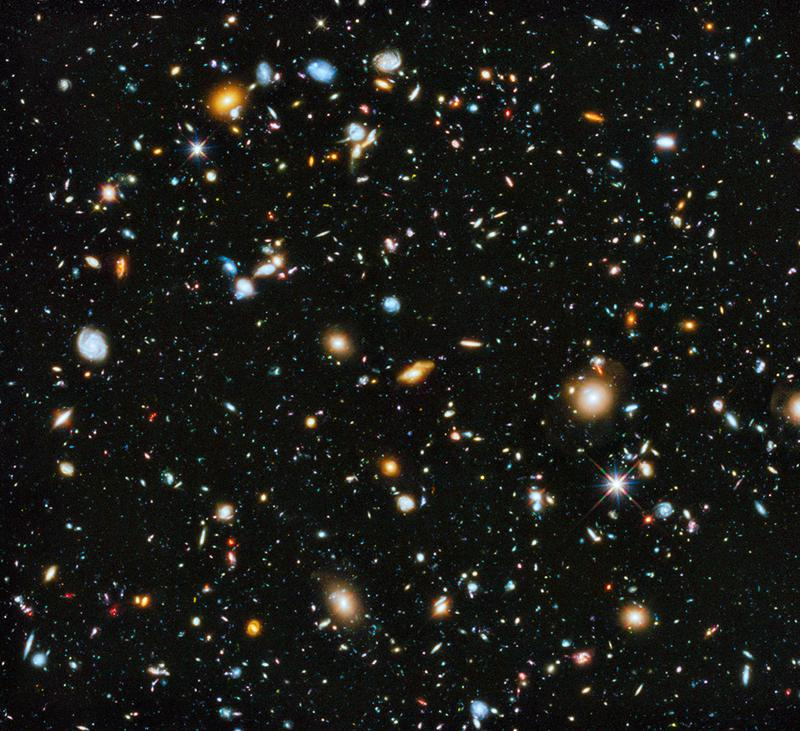
\includegraphics[width=0.9\textwidth]{hubble-ultra-deep-scaled.jpg}
            \newline
            {\tiny  Hubble Ultra Deep Field, NASA/ESA, Teplitz et al.}
        \end{center}

    }

    \definecolor{mblack}{RGB}{50,50,50}
    \setbeamertemplate{background canvas}[vertical shading][bottom=mgray,top=mblack]
}

{
    \definecolor{mblack}{RGB}{0,0,0}
    \setbeamertemplate{background canvas}[vertical shading][bottom=black,top=black]


    \frame
    {
        \begin{center}
            \includegraphics[trim=50 50 50 50,clip,width=0.75\textwidth]{CMB-Tegmark.jpeg}
        \end{center}
        {\tiny \hfill WMAP (M. Tegmark)}
    }
    \definecolor{mblack}{RGB}{50,50,50}
    \setbeamertemplate{background canvas}[vertical shading][bottom=mgray,top=mblack]

}

\frame
{
    \frametitle{Cosmology and Experiment}

    \setbeamerfont*{itemize/enumerate body}{size=\Large}
    \setbeamerfont*{itemize/enumerate subbody}{parent=itemize/enumerate body}
    \setbeamerfont*{itemize/enumerate subsubbody}{parent=itemize/enumerate body}
 
    \begin{itemize}

        \item Cosmology is driven by {\color{gold} {\em observation}} rather than {\em experimentation}
        \item We only have one universe
    \end{itemize}

}

\frame
{
    \frametitle{Cosmology and Experiment}

    \setbeamerfont*{itemize/enumerate body}{size=\Large}
    \setbeamerfont*{itemize/enumerate subbody}{parent=itemize/enumerate body}
    \setbeamerfont*{itemize/enumerate subsubbody}{parent=itemize/enumerate body}
 
    \begin{itemize}

        \item We cannot control the experiment
        \begin{itemize}
            \item At RHIC nearly identical particles are created, and the configuration
                is controlled by experimenters 
            \item We cannot create new galaxies, or start the universe over from scratch
        \end{itemize}
        \item We must {\em infer} from what already exists

        \item Then compare to theory, or derive new theories

    \end{itemize}

}


\frame
{
    \frametitle{Dark Energy}

    \setbeamerfont*{itemize/enumerate body}{size=\Large}
    \setbeamerfont*{itemize/enumerate subbody}{parent=itemize/enumerate body}
    \setbeamerfont*{itemize/enumerate subsubbody}{parent=itemize/enumerate body}
 
    \begin{itemize}

        \item A {\em purely observational} field currently, very little
            theoretical guidance
        \begin{itemize}
            \item The phenomenon is clearly detected in more than one probe
            \item But we have too little data to distinguish various 
                theoretical models
        \end{itemize}

    \end{itemize}

}



\frame
{
    \frametitle{Dark Energy Phenomenon}

    \setbeamerfont*{itemize/enumerate body}{size=\Large}
    \setbeamerfont*{itemize/enumerate subbody}{parent=itemize/enumerate body}
    \setbeamerfont*{itemize/enumerate subsubbody}{parent=itemize/enumerate body}
 
    \begin{itemize}

        \item Galaxies are flying apart (Hubble, 1920s): light is {\color{gold} {\em redshifted} }
        \item Naturally part of the Big Bang theory
        \begin{itemize}
            \item Interpret in General Relativity as the expansion of space time
        \end{itemize}

        \item Expect the rate of expansion to slow over time
        \begin{itemize}
            \item Very fast expansion at the beginning
            \item Gravity pulls everything together and slows the expansion
        \end{itemize}

    \end{itemize}

}

\frame
{
    \frametitle{Dark Energy Phenomenon}

    \setbeamerfont*{itemize/enumerate body}{size=\Large}
    \setbeamerfont*{itemize/enumerate subbody}{parent=itemize/enumerate body}
    \setbeamerfont*{itemize/enumerate subsubbody}{parent=itemize/enumerate body}
 
    \begin{itemize}

        \item We do see the expansion slowed after the Big Bang, but now it is
            speeding back up

        \begin{itemize}
            \item Type 1A Supernovae: Our best standard candles are too faint in the very distant past (1998)
            \item Baryon Acoustic Oscillations: Our best standard ruler is too big at the current time (2005)
        \end{itemize}

    \end{itemize}

}


\frame
{
    \frametitle{Example: Type 1A Supernovae}

    \setbeamerfont*{itemize/enumerate body}{size=\Large}
    \setbeamerfont*{itemize/enumerate subbody}{parent=itemize/enumerate body}
    \setbeamerfont*{itemize/enumerate subsubbody}{parent=itemize/enumerate body}
 
    \begin{center}
        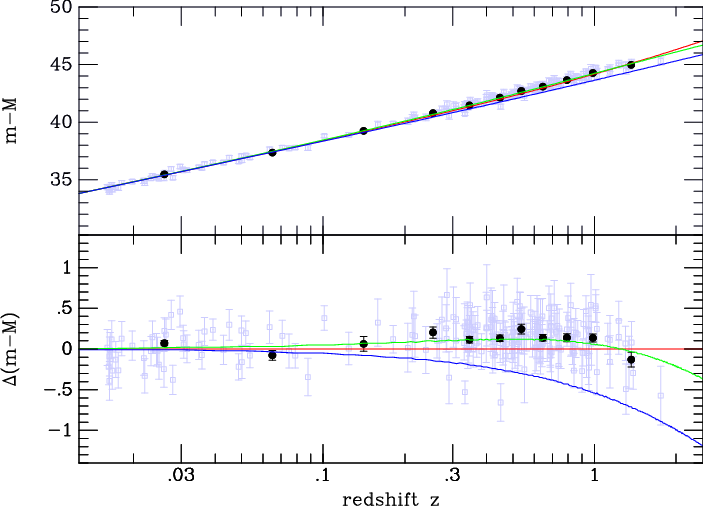
\includegraphics[width=0.8\textwidth]{davis_hub.png}
        \newline
        {\tiny Davis et al. 2007}
    \end{center}
    
    \begin{center}
        Many theories could pass through the same points: 
        \newline
        {\color{gold} Need more data!}
    \end{center}
}



{
	\definecolor{mblack}{RGB}{0,0,0}
    \setbeamertemplate{background canvas}[vertical shading][bottom=black,top=black]
	
    \frame
    {
        \frametitle{New Technique: Gravitational Lensing}

        \begin{center}
            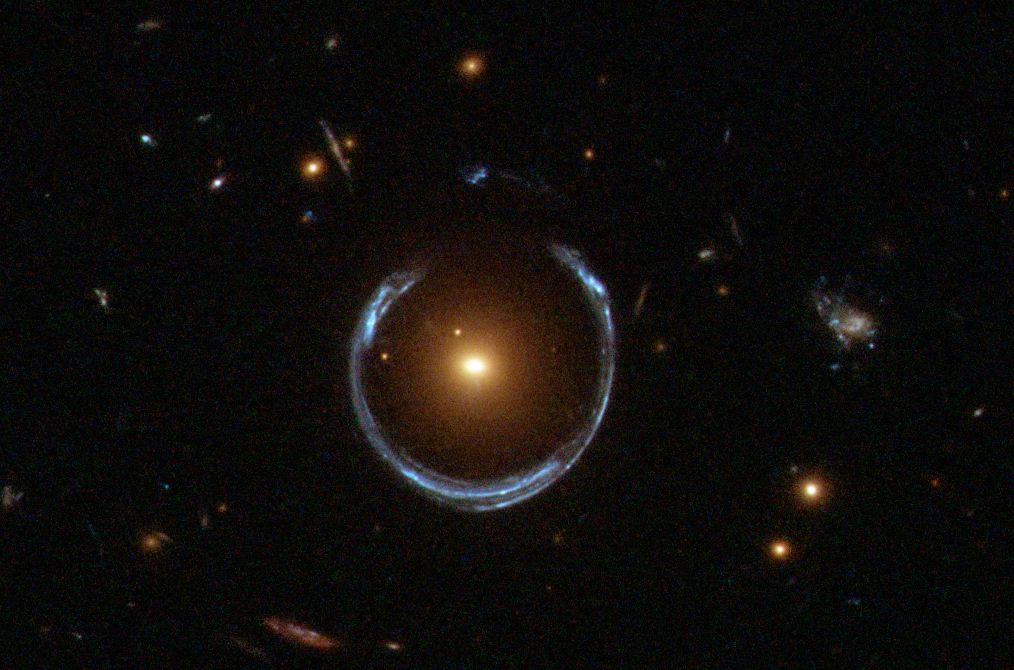
\includegraphics[height=0.7\textheight]{A_Horseshoe_Einstein_Ring_from_Hubble.JPG}

            {\tiny \hfill The ``Horseshoe'' ESA/Hubble \& NASA}
        \end{center}
    }

	\definecolor{mblack}{RGB}{50,50,50}
    \setbeamertemplate{background canvas}[vertical shading][bottom=mgray,top=mblack]

}

{
    \definecolor{mblack}{RGB}{0,0,0}
    \setbeamertemplate{background canvas}[vertical shading][bottom=black,top=black]

    \frame
    {
        \frametitle{Lensing by Galaxy Clusters: Abell 1689}

        \begin{center}
            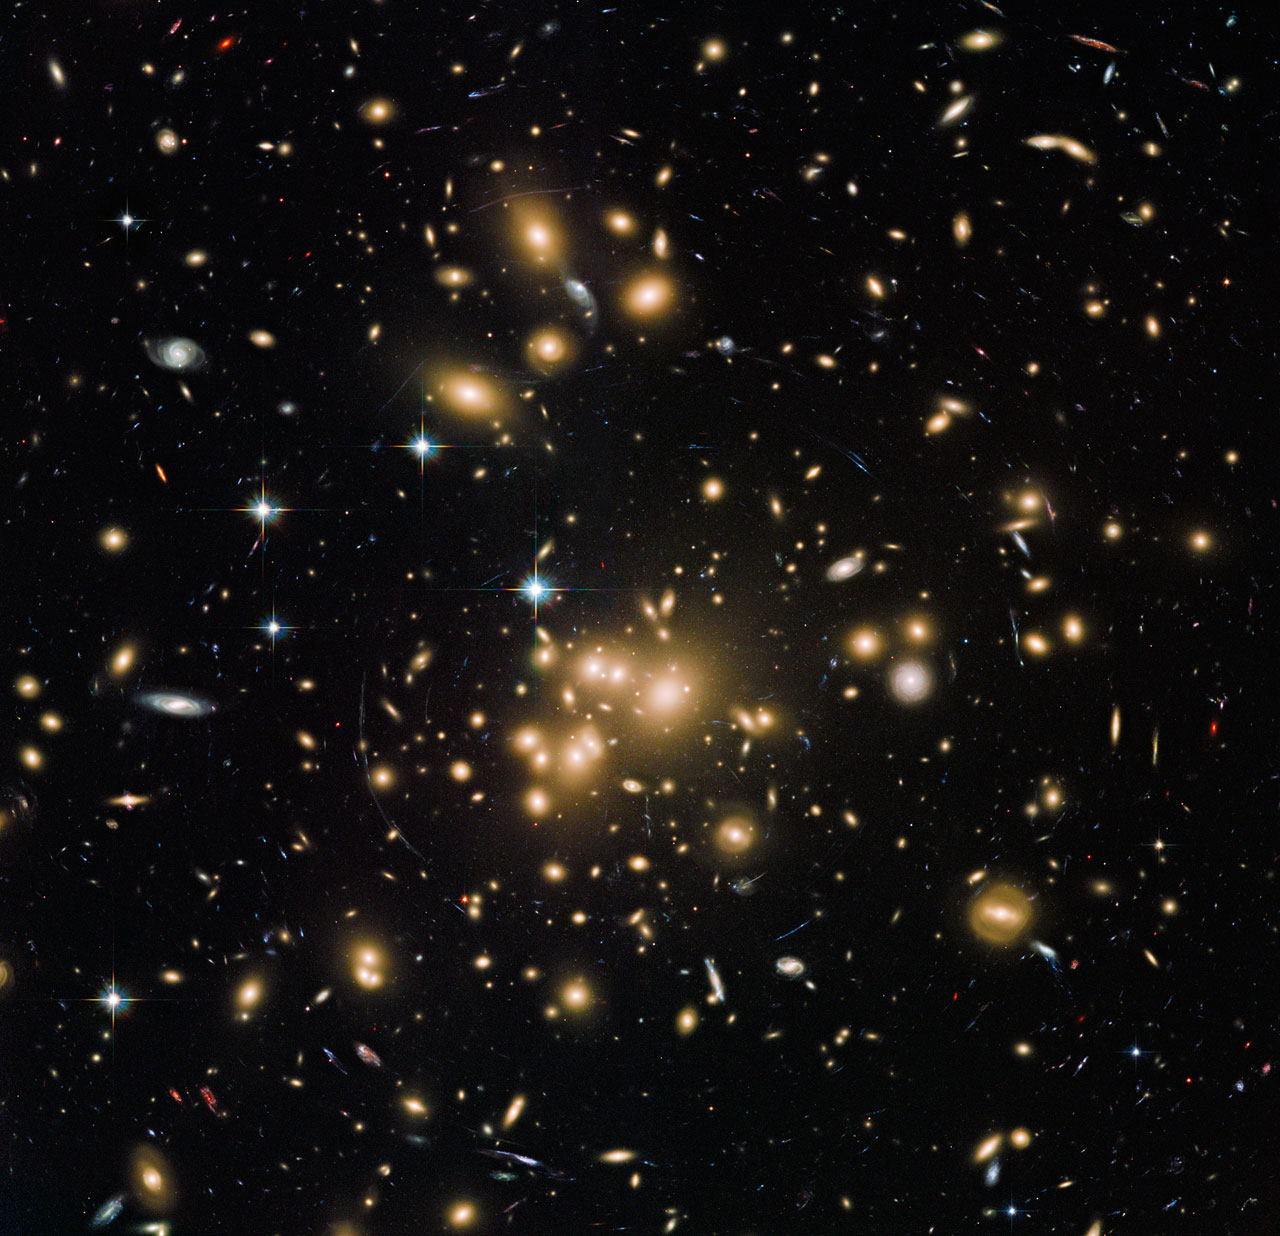
\includegraphics[height=0.8\textheight]{abell1689_hubble_1280.jpg}

            {\tiny \hfill NASA, ESA, STScI/AURA, J. Blakeslee, H. Ford}
        \end{center}
    }

    \definecolor{mblack}{RGB}{50,50,50}
    \setbeamertemplate{background canvas}[vertical shading][bottom=mgray,top=mblack]

}

{
    \definecolor{mblack}{RGB}{0,0,0}
    \setbeamertemplate{background canvas}[vertical shading][bottom=black,top=black]

    \frame
    {
        \begin{center}
            \includegraphics[height=0.9\textheight]{abell1689-details.pdf}
        \end{center}
    }

    \definecolor{mblack}{RGB}{50,50,50}
    \setbeamertemplate{background canvas}[vertical shading][bottom=mgray,top=mblack]

}


\frame
{
    \frametitle{Lensing Geometry}

    \begin{center}
        
\includegraphics[scale=0.4]{lens_geometry_invert.pdf}
        \newline
        For a point mass lens, the deflection depends on impact
        prameter and mass as
        \newline
        {\huge {\color{gold} $\alpha \propto \frac{M}{b}$ }}
    \end{center}
}

\frame
{
    \frametitle{Using Lensing to Measure Dark Energy}

    %\fontsize{9}{0.8\baselineskip}
    \begin{columns}
        \begin{column}{0.5\textwidth}    
            \begin{itemize}

                \item Lensing is geometrical, depends on the distances to all
                    components of the lens system

                \item Look at the dependence of the shear effect as a function
                    of the source redshift
                    
                \item Current lensing data does not probe a sufficent volume of
                    the universe

            \end{itemize}
        \end{column}
        \begin{column}{0.5\textwidth}
            \begin{center}
                \includegraphics[width=\textwidth]{scinv-example-invert.pdf}
            \end{center}
        \end{column}
    \end{columns}
}


\frame
{

    \frametitle{Dark Energy Survey (DES)}

    \fontsize{9}{0.8\baselineskip}

    \begin{columns}

        \begin{column}{0.4\textwidth}
            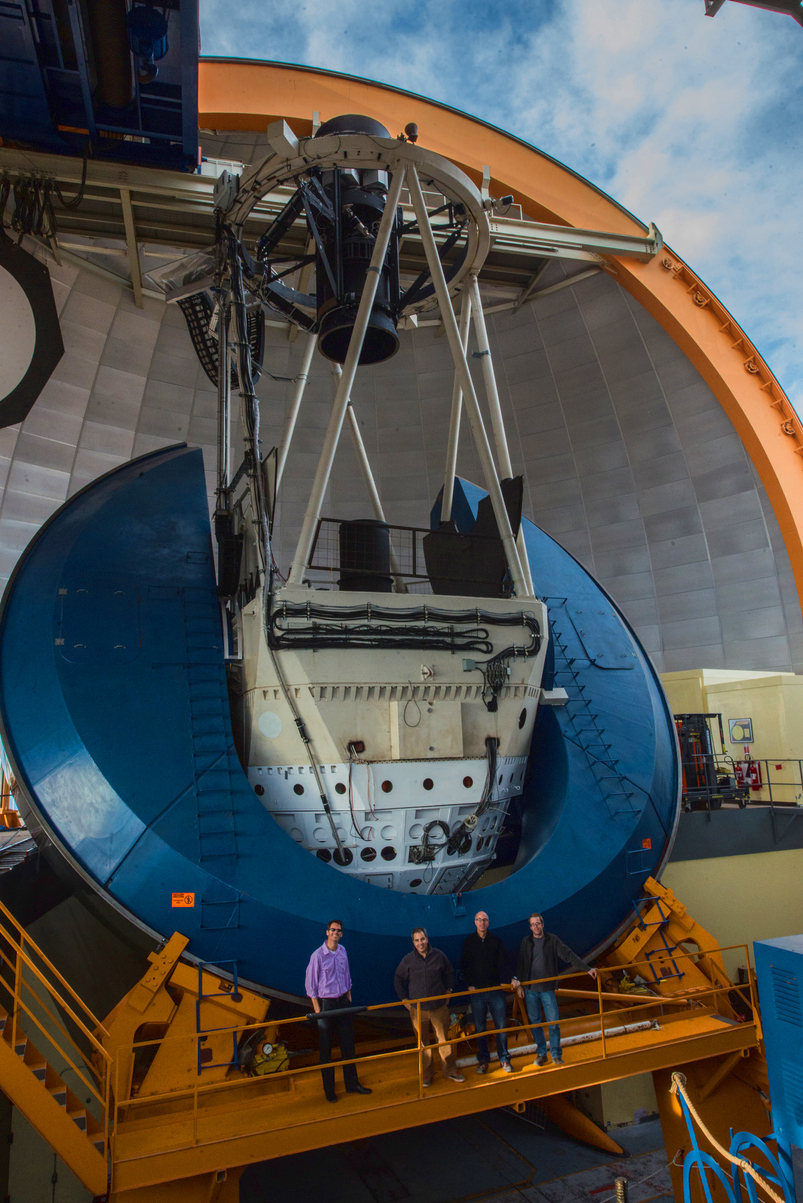
\includegraphics[scale=0.17]{ctio_blanco_crew_2013Oct-30-small-balance.jpg}
            \newline
            \hfill {\tiny Image: Brian Nord, FNAL}
        \end{column}


        \begin{column}{0.6\textwidth}

            \begin{itemize}

                \item Imaging survey of 5000 square degrees in the southern
                    sky in Chile.  5 optical filters

                \item New 500 Megapixel camera

                \item About 7 times the volume of previous largest survey: Study lensing as a
                    function of {\color{gold}cosmic time $\Rightarrow$ dark
                    energy}

                \item First light Fall 2012, survey start Aug. 31, 2013, end 2018.

                \item Study Dark Energy using weak lensing, galaxy clusters,
                    large scale structure and supernovae.

                \item Constrain Dark Energy models to {\color{gold} 2\%}

            \end{itemize}

        \end{column}

    \end{columns}

}

{
	\definecolor{mblack}{RGB}{0,0,0}
    \setbeamertemplate{background canvas}[vertical shading][bottom=black,top=black]
	
    \frame
    {

        \begin{center}
            %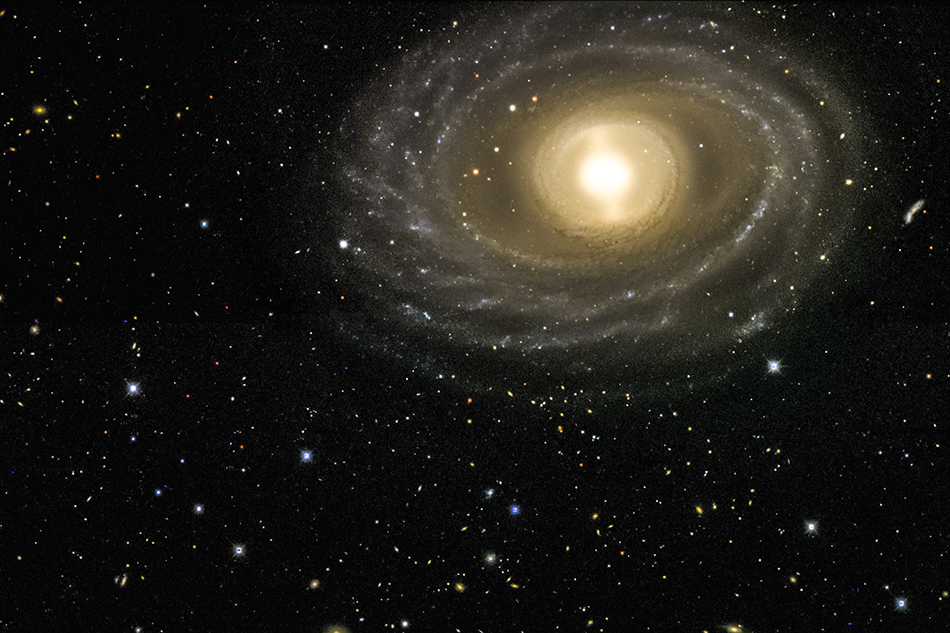
\includegraphics[width=1.1\textwidth]{ngc_new_v0-1398_20130130-mm1-2-950px.jpg}
            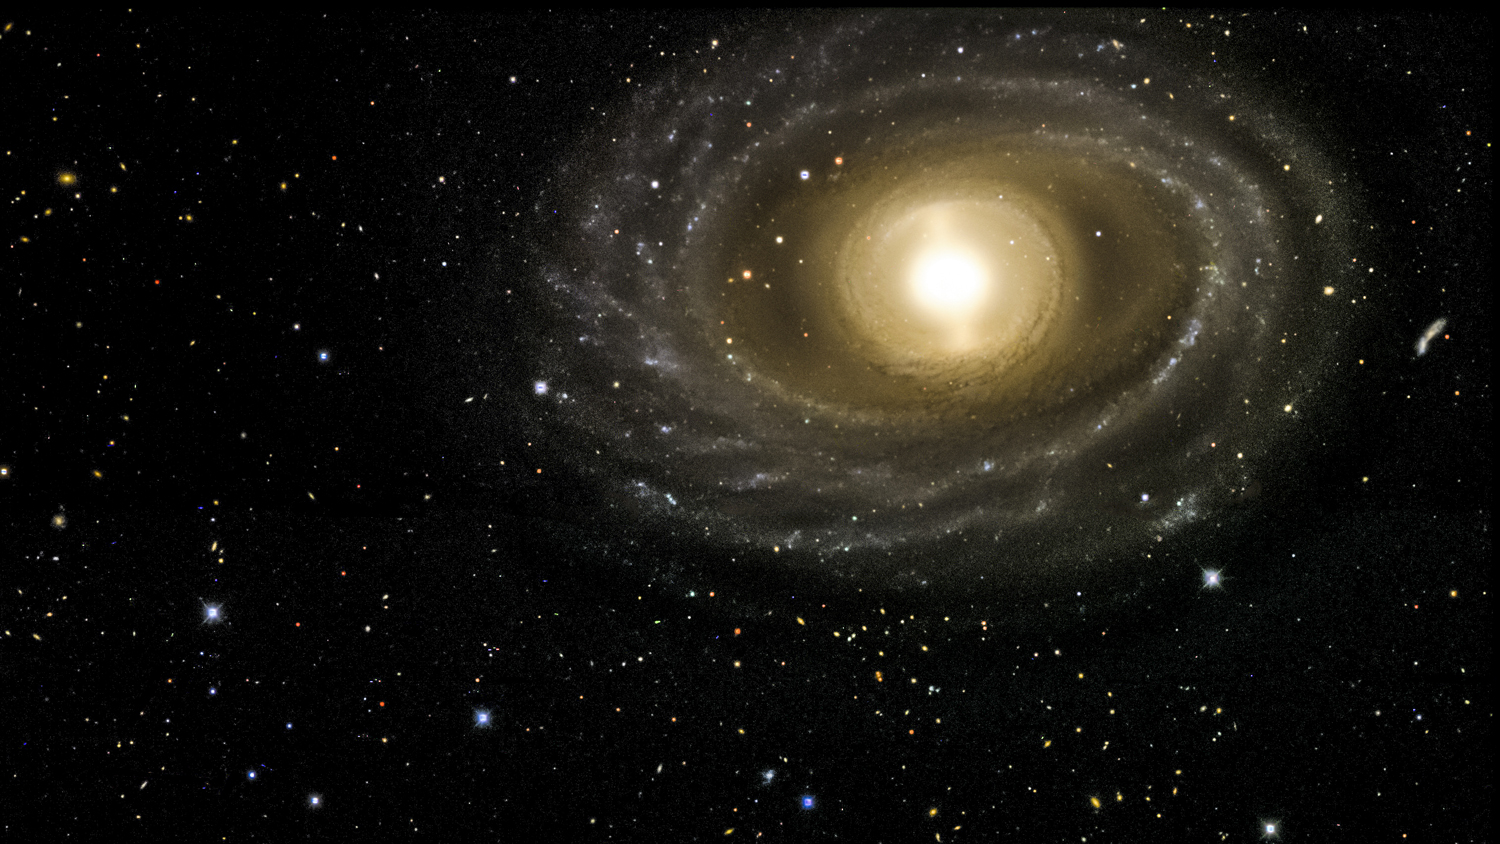
\includegraphics[width=1.1\textwidth]{DES-2013-01-medres.jpg}

            {\tiny \hfill NGC 1398, Erin Sheldon, Martin Murphy}
        \end{center}
    }

	\definecolor{mblack}{RGB}{50,50,50}
    \setbeamertemplate{background canvas}[vertical shading][bottom=mgray,top=mblack]

}

\frame
{

    \frametitle{DES at BNL}

    \setbeamerfont*{itemize/enumerate body}{size=\small}
    \setbeamerfont*{itemize/enumerate subbody}{parent=itemize/enumerate body}
    \setbeamerfont*{itemize/enumerate subsubbody}{parent=itemize/enumerate body}
 
    \begin{columns}
        \begin{column}{0.5\textwidth}    
            \begin{itemize}

                \item I've been working on DES since 2003

                \item I am a {\color{gold} builder} and {\color{gold} associate
                    member} with data rights for self, postdoc, students.

                \item Co-convener of weak lensing working group

                \item Responsible for one of the two lensing codes

                \item Leading the effort to measure lensing around galaxy clusters

            \end{itemize}
        \end{column}
        \begin{column}{0.5\textwidth}
                \centering
                %\newline
                %\includegraphics[width=\textwidth]{ngc0894-rebin4.jpg}
                %\newline
                %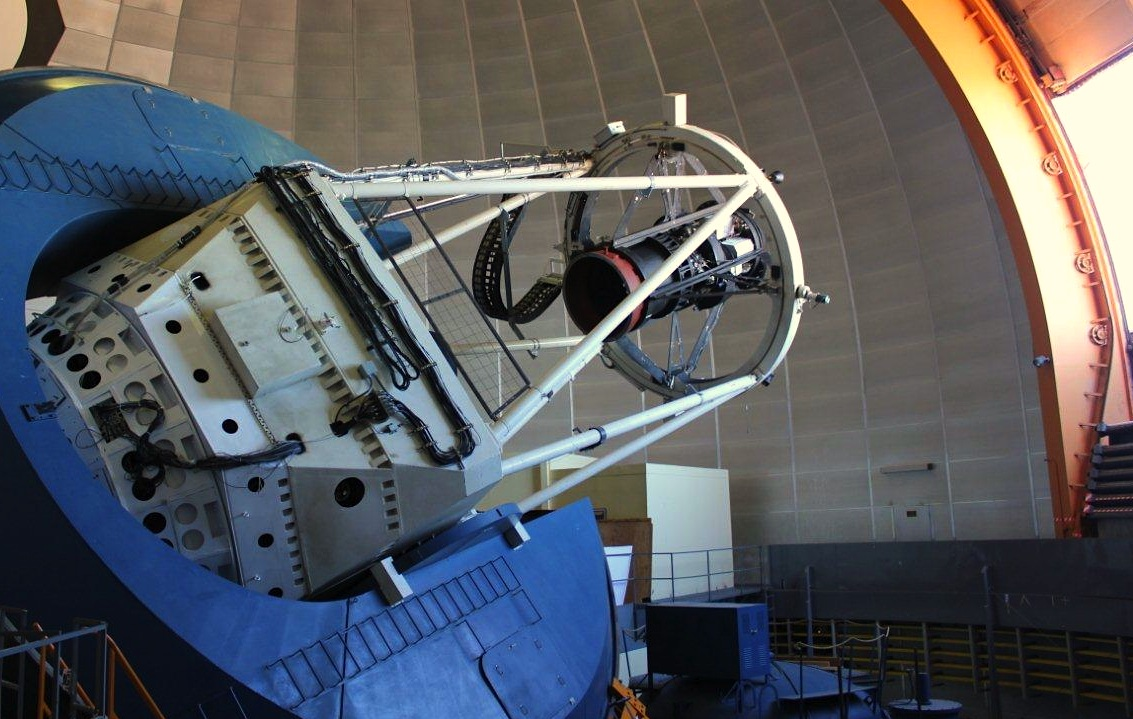
\includegraphics[width=\textwidth]{decam-image-1-medres-crop.jpg}
                %\newline
                %{\tiny Camera Installation}
                \includegraphics[angle=90,origin=c,height=0.6\textheight,trim=0 0 200 0,clip]{ngc0894-rebin4.jpg}
                \newline
                {\tiny Image: Erin Sheldon}
        \end{column}
    \end{columns}

}


\frame
{

    \frametitle{Early DES Lensing Results}
 
    \setbeamerfont*{itemize/enumerate body}{size=\Large}
    \setbeamerfont*{itemize/enumerate subbody}{parent=itemize/enumerate body}
    \setbeamerfont*{itemize/enumerate subsubbody}{parent=itemize/enumerate body}
 
    \begin{itemize}

        \item In 2015 we released our first set of papers

        \item Using very early data, only 3\% of final data set

        \item All studies used my lensing measurements, plus measurements
            from another ``competing'' group.

    \end{itemize}

}


\frame
{

    \frametitle{Early DES Lensing Highlights: Mass Mapping}

    \setbeamerfont*{itemize/enumerate body}{size=\small}
    \setbeamerfont*{itemize/enumerate subbody}{parent=itemize/enumerate body}
    \setbeamerfont*{itemize/enumerate subsubbody}{parent=itemize/enumerate body}
 
    \begin{columns}
        \begin{column}{0.4\textwidth}
            \begin{itemize}

                \item ``Mass mapping'': infer the projected mass density
                    over the entire DES data set
                
                \item Mass is dominated by dark matter.

                \item We see a good correlation between these mass structures
                    and the distribution of galaxies and clusters

            \end{itemize}
        \end{column}
        \begin{column}{0.6\textwidth}
                \centering
                %\newline
                %\includegraphics[width=\textwidth]{ngc0894-rebin4.jpg}
                %\newline
                %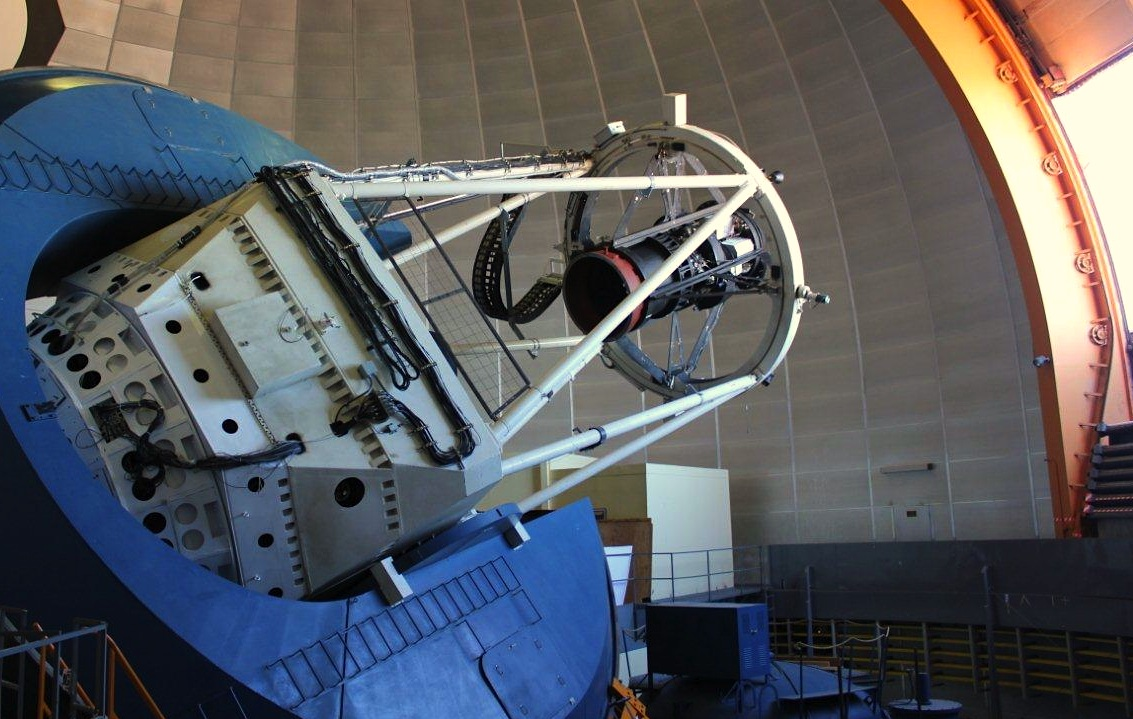
\includegraphics[width=\textwidth]{decam-image-1-medres-crop.jpg}
                %\newline
                %{\tiny Camera Installation}
                %\includegraphics[angle=90,origin=c,height=0.6\textheight,trim=0 0 200 0,clip]{ngc0894-rebin4.jpg}
                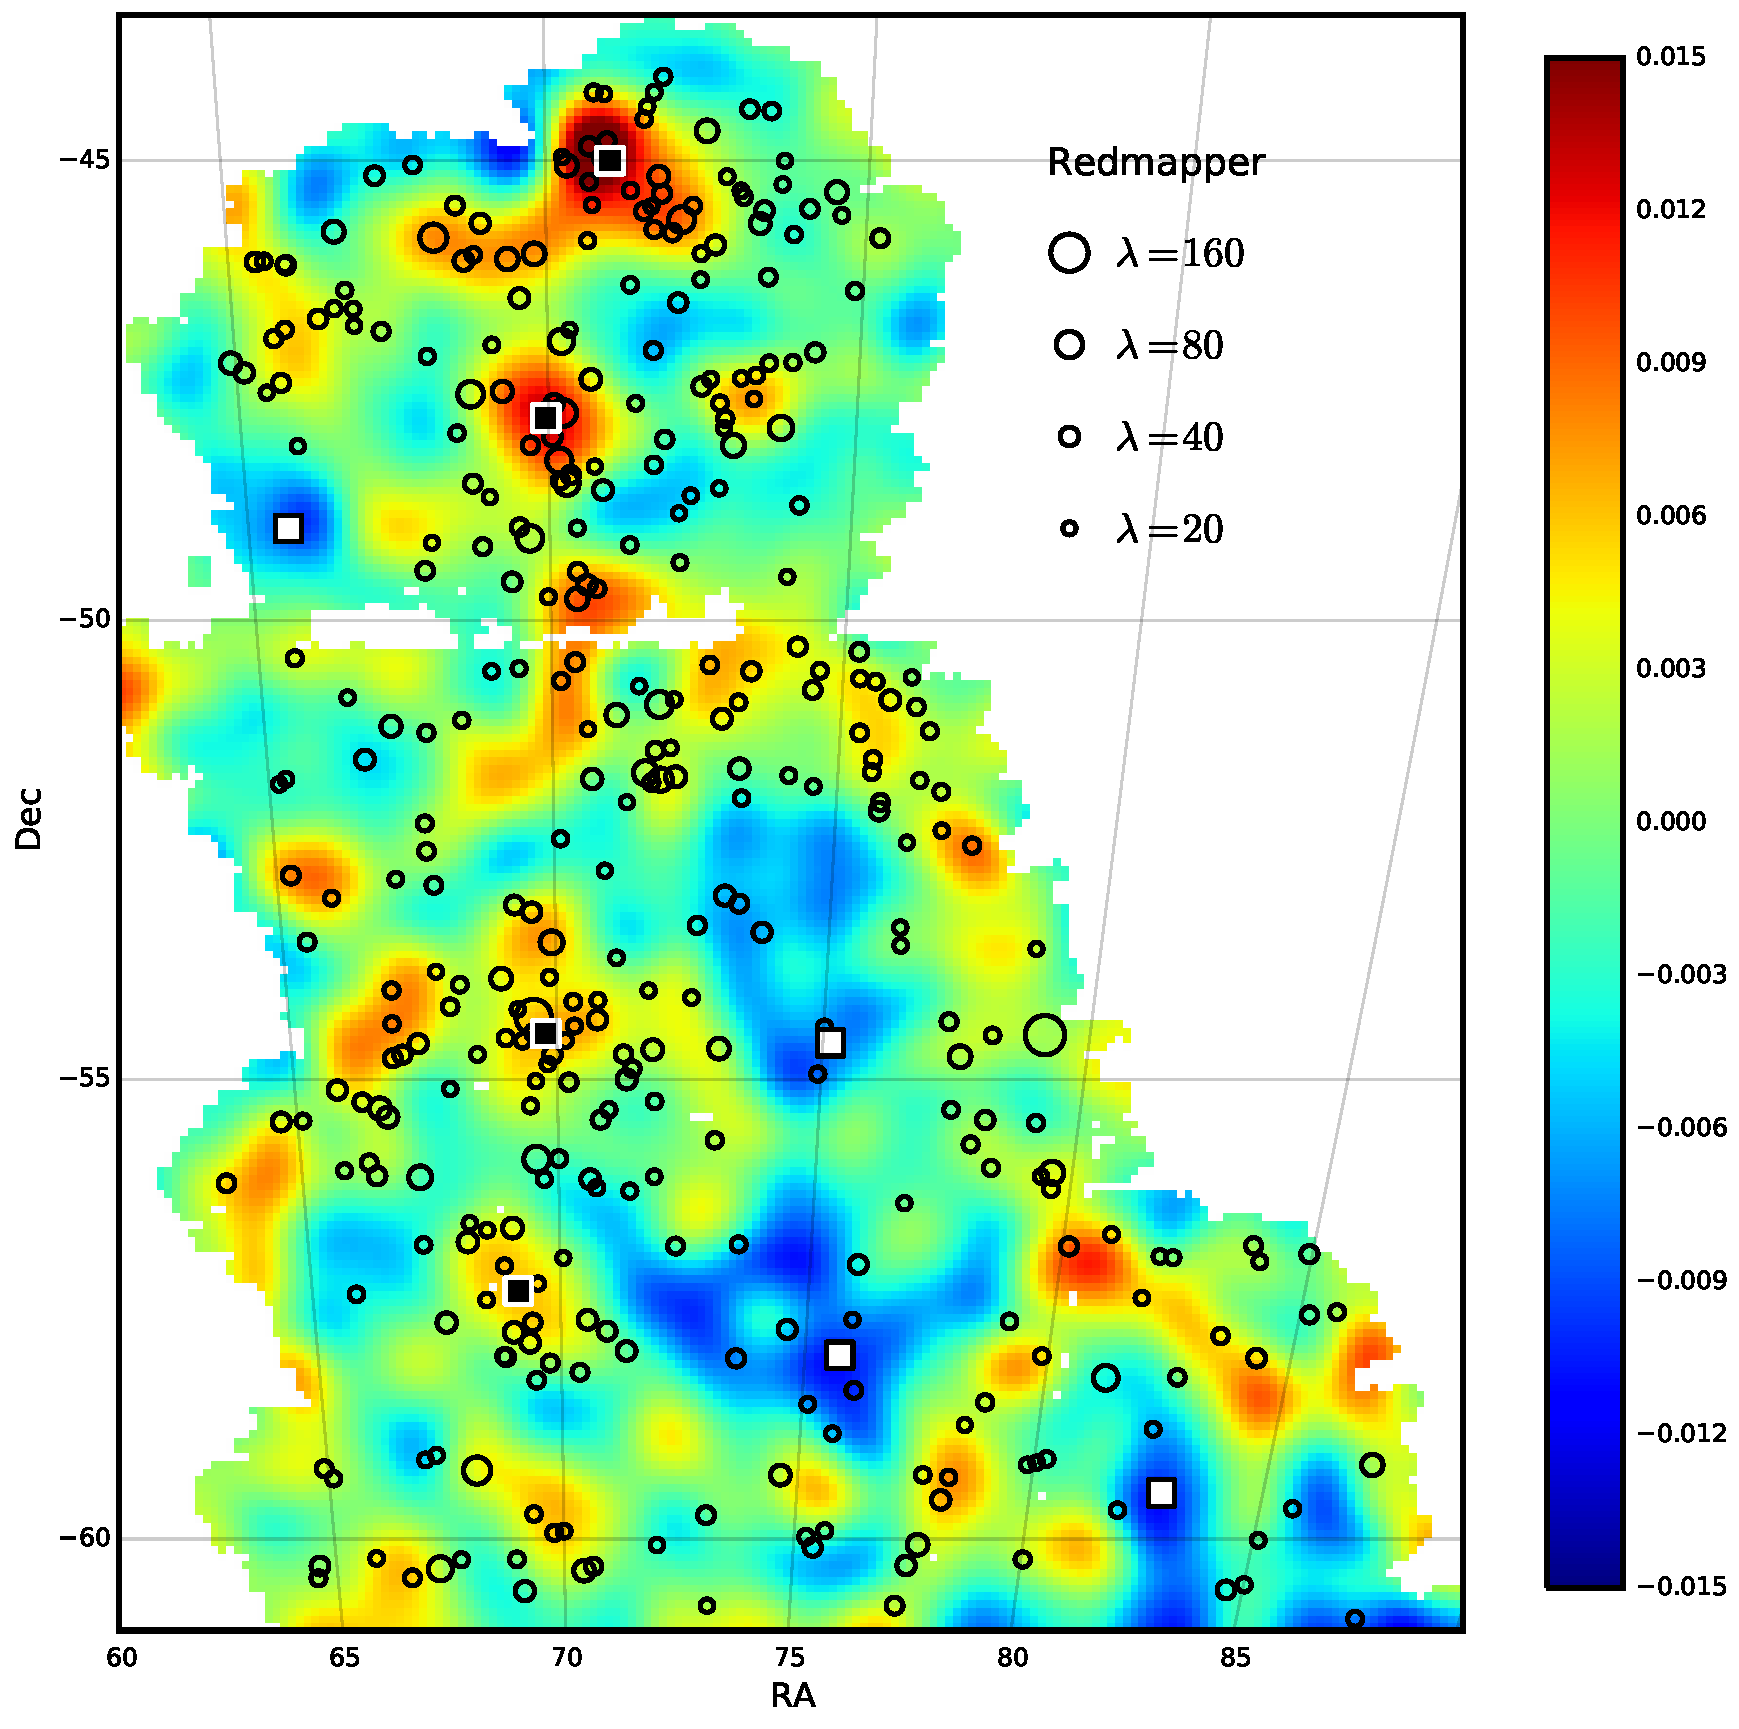
\includegraphics[width=\textwidth]{cluster_overlay_ngmix_bpz.pdf}
                \newline
                {\tiny Chang et al. 2015}
        \end{column}
    \end{columns}

}

\frame
{

    \frametitle{Early DES Lensing Highlights: Dark Matter Correlations}

    \setbeamerfont*{itemize/enumerate body}{size=\small}
    \setbeamerfont*{itemize/enumerate subbody}{parent=itemize/enumerate body}
    \setbeamerfont*{itemize/enumerate subsubbody}{parent=itemize/enumerate body}
 
    \begin{columns}
        \begin{column}{0.4\textwidth}
            \begin{itemize}

                \item Correlation function of Dark Matter
                
                \item Predicted by theory

                \item Dark Matter is strongly correlated, in agreement with predictions

                \item Details depend on Dark Energy as well

            \end{itemize}
        \end{column}
        \begin{column}{0.6\textwidth}
                \centering
                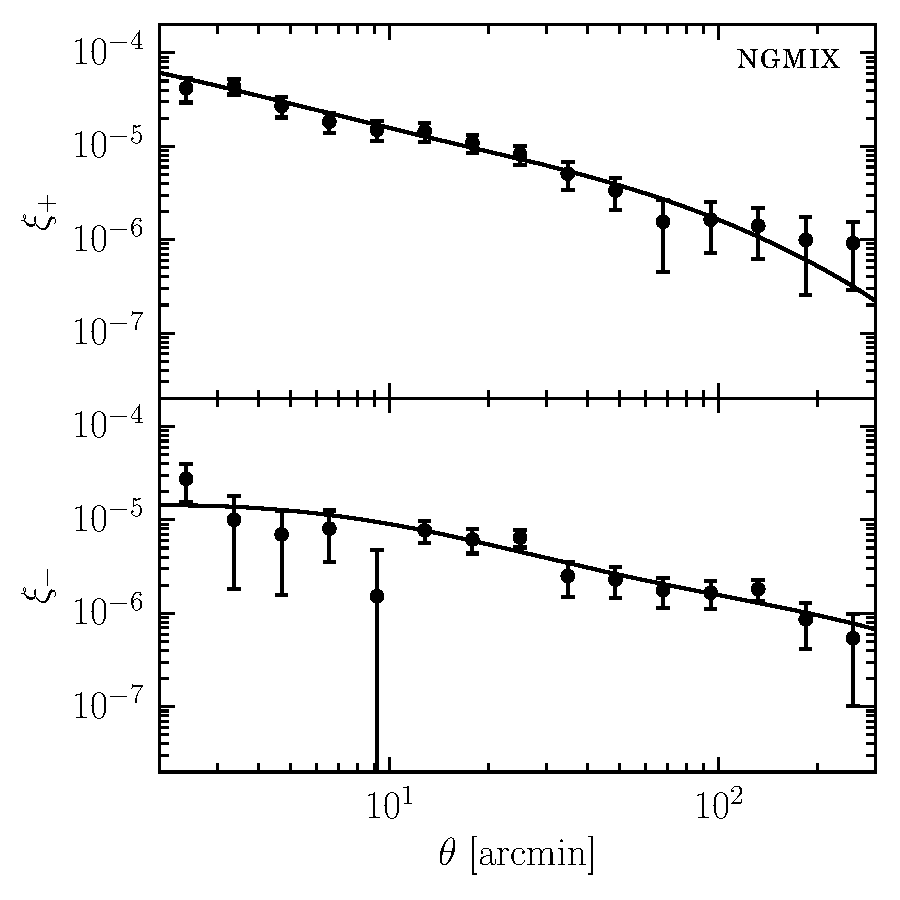
\includegraphics[width=\textwidth]{ngmix_xi.pdf}
                \newline
                {\tiny Becker et al. 2015}
        \end{column}
    \end{columns}

}

\frame
{

    \frametitle{Early DES Lensing Highlights: Cosmological Parameters}

    \setbeamerfont*{itemize/enumerate body}{size=\small}
    \setbeamerfont*{itemize/enumerate subbody}{parent=itemize/enumerate body}
    \setbeamerfont*{itemize/enumerate subsubbody}{parent=itemize/enumerate body}
 
    \begin{columns}
        \begin{column}{0.4\textwidth}
            \begin{itemize}

                \item Early data (3\% of final), not enough to constrain Dark Energy
                
                \item We do constrain the amount of dark matter in the universe, and
                    its clustering properties

                \item Best combination: dark matter density times r.m.s. fluctuation
                    of mass density

            \end{itemize}
        \end{column}
        \begin{column}{0.6\textwidth}
                \centering
                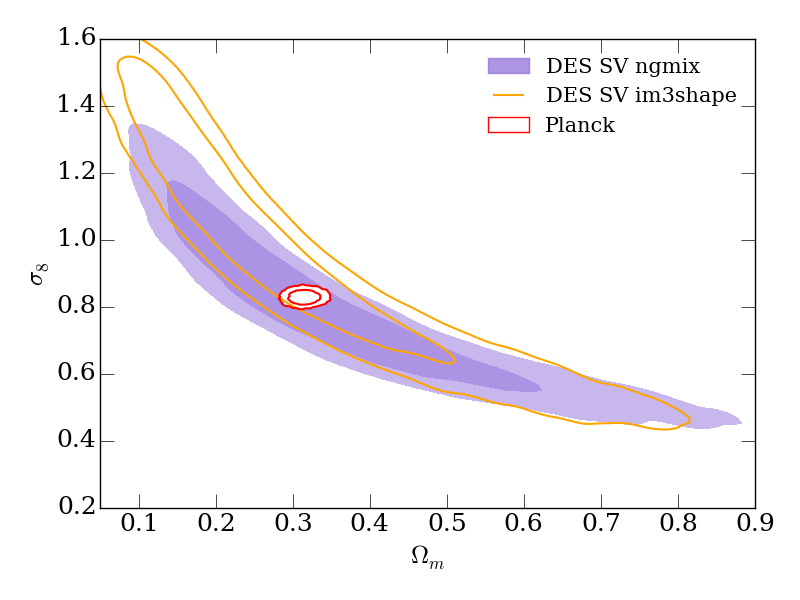
\includegraphics[width=\textwidth]{Om_sig8_im3.png}
                \newline
                {\tiny DES Collaboration, 2015}
        \end{column}
    \end{columns}

}


\frame
{

    \frametitle{Current and Future Work}
 
    \setbeamerfont*{itemize/enumerate body}{size=\Large}
    \setbeamerfont*{itemize/enumerate subbody}{parent=itemize/enumerate body}
    \setbeamerfont*{itemize/enumerate subsubbody}{parent=itemize/enumerate body}
 
    \begin{itemize}


        \item I'm currently working on lensing by specific objects found in
            DES: Clusters of Galaxies, the largest structures in the universe.

        \begin{itemize}
            \item Very high signal, compared to the correlation function analysis.
        \end{itemize}

        \item New lensing measurement code
        \begin{itemize}
            \item Current code accurate to $\sim 2$\%.
            \item New code accurate to better than 0.1\%, good enough for
                requirements of DES and future surveys.
        \end{itemize}

        \item Take and analyze more data!

    \end{itemize}

}




\frame
{

    \frametitle{Summary}
 
    \setbeamerfont*{itemize/enumerate body}{size=\Large}
    \setbeamerfont*{itemize/enumerate subbody}{parent=itemize/enumerate body}
    \setbeamerfont*{itemize/enumerate subsubbody}{parent=itemize/enumerate body}
 
    \begin{itemize}

        \item Gravitational lensing is a promising probe of Dark Energy

        \item The Dark Energy Survey is under way

        \item Expect groundbreaking results on Dark Energy in coming years

    \end{itemize}

}





\end{document}
